\documentclass[]{article}
\newcommand{\FileDepth}{../../..}
\usepackage[letterpaper, landscape, margin=0.5cm]{geometry}
\usepackage[T1]{fontenc}
\usepackage{textcomp}%Not strictly necessary, but gives \textmu command for "micro."
\usepackage{fancyhdr}
\usepackage{amsmath}
\usepackage{amssymb}
\usepackage{graphicx}
\usepackage{xcolor}
\usepackage{tikz}
\usetikzlibrary{calc}
\usepackage[shortlabels]{enumitem}
\usepackage{multicol}
\usepackage{vwcol}
\usepackage{hyperref}
\usepackage{wrapfig}
%opening
\newcommand{\SecType}{S}
\newcommand{\Week}{4}
\title{PH 211 Studio \Week}
\author{Benjamin Bauml}
\date{Summer 2024}

\newcommand{\Purpose}{4}
\newcommand{\DefOnly}{0}

\input{\FileDepth/Formats/Assignment20240614.tex}
\usepackage[absolute]{textpos}
% This package relies on Assignment Format 2024-06-14 or later to work. It is recommended that the Purpose and DefOnly commands be given as such:
%\newcommand{\Purpose}{4}
%\newcommand{\DefOnly}{0}
% Activities need to be entered outside of the TeacherMargin and PresentSpace environments, otherwise they will be defined only locally. They can even go in the preamble.
\newenvironment{TeacherMargin}{\begin{textblock*}{10.8cm}(0.5cm,0.5cm)
\small}{\end{textblock*}
\hspace{0.1cm}}
\newenvironment{PresentSpace}{\begin{textblock*}{0.3cm}(26.85cm,9.35cm)
--
\end{textblock*}
\begin{textblock*}{15.6cm}(11.8cm,0.5cm)
\begin{Repurpose}{1}
\Large}{\end{Repurpose}
\end{textblock*}
\hspace{0.1cm}}

\newcommand{\FBDaxes}[4][2]{
	\begin{scope}[shift={(#2)},rotate=#3]
		% x-axis
		\draw[thick,->] (-#1,0) -- (#1,0);
		\node[anchor=west] at (#1,0) {$x$};
		% y-axis
		\draw[thick,->] (0,-#1) -- (0,#1);
		\node[anchor=south] at (0,#1) {$y$};
		\coordinate (#4) at (0,0);
	\end{scope}
}
\newcommand{\FBDvectorMA}[4]{
	\begin{scope}[shift={(#1)}]
		\coordinate (#4tip) at ({#2*cos(#3)},{#2*sin(#3)});
		\draw[ultra thick,blue,->] (#1) -- (#4tip);
	\end{scope}
}
\newcommand{\FBDvectorXY}[3]{
	\begin{scope}[shift={(#1)}]
		\coordinate (#3tip) at (#2);
		\draw[ultra thick,blue,->] (0,0) -- (#3tip);
	\end{scope}
}
\newcommand{\FBDdot}[1]{
	\filldraw[black] (#1) circle (3pt);
}
\newcommand{\FBDbox}[5][1]{
	\begin{scope}[shift={(#2)},rotate=#3]
		\filldraw[color=black,fill=white,thick] ({-#1/2},{#1/2}) -- ({-#1/2},{-#1/2}) -- ({#1/2},{-#1/2}) -- ({#1/2},{#1/2}) -- cycle;
		% Left side coordinates
		\coordinate (#4ltq) at ({-#1/2},{#1/4});
		\coordinate (#4lcent) at ({-#1/2},0);
		\coordinate (#4lbq) at ({-#1/2},{-#1/4});
		% right side coordinates
		\coordinate (#4rtq) at ({#1/2},{#1/4});
		\coordinate (#4rcent) at ({#1/2},0);
		\coordinate (#4rbq) at ({#1/2},{-#1/4});
		% top coordinates
		\coordinate (#4tlq) at ({-#1/4},{#1/2});
		\coordinate (#4tcent) at (0,{#1/2});
		\coordinate (#4trq) at ({#1/4},{#1/2});
		% bottom coordinates
		\coordinate (#4blq) at ({-#1/4},{-#1/2});
		\coordinate (#4bcent) at (0,{-#1/2});
		\coordinate (#4brq) at ({#1/4},{-#1/2});
		% corners
		\coordinate (#4tl) at ({-#1/2},{#1/2});
		\coordinate (#4tr) at ({#1/2},{#1/2});
		\coordinate (#4bl) at ({-#1/2},{-#1/2});
		\coordinate (#4br) at ({#1/2},{-#1/2});
		\node at (0,0) {#5};
	\end{scope}
}
%\newcommand{\MVec}[3][0]{%Creates a momentum vector of length #3 centered at #2 and rotated #1 degrees counterclockwise.
	\begin{scope}[rotate=#1,shift={(#2)}]
		\draw[->,thick] ({-#3/2},0) -- ({#3/2},0);
	\end{scope}
}
\newcommand{\MDot}[1]{%Creates a dot at #1 to represent a zero vector.
	\filldraw (#1) circle (1pt);
}
\newcommand{\MVDRows}[2][4.5]{%Creates the rows (initial, delta, final) of a momentum vector diagram. The optional argument determines the width of the table, and defaults to a good length for three columns (two objects and the total system). The non-optional argument gives a coordinate name (not displayed) to the diagram.
	\begin{scope}
		%\draw[thick] (0,5.5) -- (0,0);
		\draw[thick] (-1,4.5) -- (#1,4.5);
		\node at (-0.5,3.75) {$\vec{p}_{i}$};
		\draw[thick] (-1,3) -- (#1,3);
		\node at (-0.5,2.25) {$\Delta\vec{p}$};
		\draw[thick] (-1,1.5) -- (#1,1.5);
		\node at (-0.5,0.75) {$\vec{p}_{f}$};
		\coordinate (#2) at (0,5);
	\end{scope}
}
\newcommand{\MVDCol}[4][0.75]{%Creates a column for an object in a momentum vector diagram. The first (non-optional) argument is the coordinate name (not displayed) of the column, while the second is the displayed column header. The first argument also names the three entries down the column. The third argument anchors the column, so it should either be the coordinate name of the MVD (for the first column) or the coordinate name of the previous column. The optional argument indicates how far the center of the column should be from the previous column's edge, and defaults to 0.75.
	\begin{scope}[shift={(#4)}]
		\node at (#1,0) {#3};
		%\draw[thick] ({#1*2},0.5) -- ({#1*2},-5);
		\draw[thick] (0,0.5) -- (0,-5);
		\coordinate (#2init) at (#1,-1.25);
		\coordinate (#2delt) at (#1,-2.75);
		\coordinate (#2fin) at (#1,-4.25);
		\coordinate (#2) at ({#1*2},0);
	\end{scope}
}

%\input{\FileDepth/Activities/Activity_One/Activity_One.tex}
%\input{\FileDepth/Activities/Activity_Two/Activity_Two.tex}

\begin{document}
\begin{TeacherMargin}

\end{TeacherMargin}
\begin{PresentSpace}
\begin{center}
	\huge Studio 4: Gravity and Friction \\
	\vspace{1cm}
\end{center}
\underline{Warm-Up Activity} \\
%How do you feel about the quizzes? Which of the following is the magnitude of the friction on the book at the front of the room?
\begin{comment}{2}
\begin{enumerate}[(A)]
	\item Velocity is acceleration times $t$.
	\vspace{6pt}
	\item Acceleration is velocity times $t$.
	\vspace{15pt}
	\item Acceleration is the derivative of velocity.
	\item Velocity is the derivative of acceleration.
\end{enumerate}
\end{comment}
\end{PresentSpace}
\newpage
\begin{TeacherMargin}

\end{TeacherMargin}
\begin{PresentSpace}
\vspace{-10pt}
\section*{(Newton's) Laws of Motion}
\vspace{-10pt}
\begin{enumerate}[(1)]
	\item An object in motion (or at rest) stays in motion (or at rest) unless a net external force acts on it.
	\item The net force on an object is equal to the object's mass times its acceleration:
	\[
	\vec{F}^{net} = m\vec{a}.
	\]
	\item If A exerts a force on B, then B exerts a force of the same magnitude on A in the opposite direction:
	\[
	\vec{F}_{AB} = -\vec{F}_{BA}.
	\]
\end{enumerate}
\end{PresentSpace}
\newpage
\begin{TeacherMargin}

\end{TeacherMargin}
\begin{PresentSpace}
\vspace{-10pt}
\section*{Types of Forces}
\vspace{-10pt}
\begin{itemize}
	\item Gravity \qquad \qquad \qquad \qquad $\vec{F}^{g}_{AB} = m_{A}\vec{g}_{B}$
	\begin{itemize}
		\item Newtonian \qquad\ $\vec{g}_{B} = G\frac{M_{B}}{r^{2}}(-\hat{r})$, $G = 6.67408\times10^{-11}\text{ N}\cdot\text{m}^{2}/\text{kg}^{2}$
		\item Near-Earth \qquad $\vec{g}_{E} = g(-\hat{y}),\ g=9.81\frac{\text{m}}{\text{s}^{2}} \approx 10\frac{\text{m}}{\text{s}^{2}}$
	\end{itemize}
	\item Normal \qquad $\vec{F}^{N}$ always $\bot$; varies in magnitude
	\item Tension \qquad $\vec{F}^{T}$ uniform (massless, inextensible rope)
	\item Spring
	\item Friction
	\begin{itemize}
		\item Static Friction \qquad $F^{sf}\leq\mu_{s}|\vec{F}^{N}|$
		\item Kinetic Friction \qquad $F^{kf}=\mu_{k}|\vec{F}^{N}|$
	\end{itemize}
\end{itemize}
\end{PresentSpace}
\newpage
\begin{TeacherMargin}

\end{TeacherMargin}
\begin{PresentSpace}
\vspace{-10pt}
\section*{S4-1: The Elevator}
\vspace{-10pt}
\begin{itemize}
	\item You attach a volleyball with mass 275 grams to a string and suspend it from the ceiling of an elevator.
	\item The elevator is moving upward at constant speed 1.5 m/s.
	\item Our goal is to determine the tension in the string.
	\begin{itemize}
		\item Choose a system and identify any assumptions you are making.
		\item Sketch and label a free body diagram.
		\item Determine the tension.
		\item Make sense of your answer.
	\end{itemize}
\end{itemize}
\end{PresentSpace}
\newpage
\begin{TeacherMargin}

\end{TeacherMargin}
\begin{PresentSpace}
\vspace{-10pt}
\section*{S4-2: The Accelerating Elevator}
\vspace{-10pt}
\begin{itemize}
	\item You attach a volleyball with mass 275 grams to a string and suspend it from the ceiling of an elevator.
	\item The elevator is moving upward at constant speed 1.5 m/s and accelerating upward at a constant rate of 2.5 m/s$^{2}$.
	\begin{itemize}
		\item Do you want to change your system or assumptions?
		\item How (if at all) does your free body diagram change?
		\item How (if at all) does the tension change?
	\end{itemize}
\end{itemize}
\end{PresentSpace}
\newpage
\begin{TeacherMargin}

\end{TeacherMargin}
\begin{PresentSpace}
\vspace{-10pt}
\section*{S4-3: The Space Elevator}
\vspace{-10pt}
\begin{itemize}
	\item You attach a volleyball with mass 275 grams to a string and suspend it from the ceiling of an elevator.
	\item The elevator is located 400 km above the surface of the Earth and moving upward at constant speed.
	\begin{itemize}
		\item Do you want to change your system or assumptions?
		\item How (if at all) does your free body diagram change?
		\item How (if at all) does the tension change?
	\end{itemize}
\end{itemize}
\end{PresentSpace}
\newpage
\begin{TeacherMargin}

\end{TeacherMargin}
\begin{PresentSpace}
\vspace{-10pt}
\section*{S4-4: The Crate on Top of the Truck I (Gaining Speed)}
\vspace{-10pt}
\begin{itemize}
	\item A truck is initially moving to the right with speed $v_{i}$.
	\item The driver left a crate on top of the truck. We know the mass of the crate ($m_{c}$) and the coefficients of friction ($\mu_{s}$ and $\mu_{k}$).
	\item The truck begins \textit{speeding up}, but the driver wants to prevent the crate from sliding.
	\begin{itemize}
		\item Draw a free-body diagram for the crate.
		\begin{itemize}
			\item What kind of friction acts on the crate?
			\item What direction is the force of friction?
		\end{itemize}
		\item What do we know about the truck's
		\begin{itemize}
			\item velocity?
			\item acceleration?
		\end{itemize}
	\end{itemize}
\end{itemize}
\end{PresentSpace}
\begin{textblock*}{5cm}(22cm,3cm)
\centering
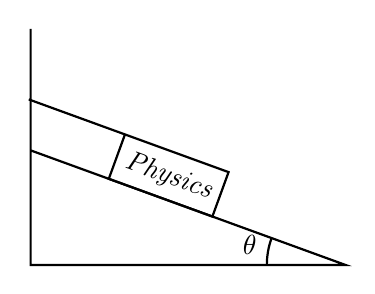
\begin{tikzpicture}
	\draw[thick] (-4,3) -- (-4,0) -- (0,0) -- (-4,{4*tan(20)});
	\draw[thick] (-1,0) node[anchor=south east] {$\theta$} arc (180:160:1);
	\draw[thick,rotate=-20] (-3.2,0) node[anchor=south west,rotate=-20] {\textit{Physics}} rectangle (-1.8,0.6);
	\draw[thick,rotate=-20] (-3.2,0.6) -- (-4.5,0.6);
\end{tikzpicture}
\end{textblock*}
\newpage
\begin{TeacherMargin}

\end{TeacherMargin}
\begin{PresentSpace}
\vspace{-10pt}
\section*{S4-5: The Crate on Top of the Truck II (Slamming on the Brakes)}
\vspace{-10pt}
\begin{itemize}
	\item A truck is initially moving to the right with speed $v_{i}$.
	\item We know the mass of the crate ($m_{c}$) and the coefficients of friction ($\mu_{s}$ and $\mu_{k}$).
	\item The driver suddenly has to slam on the brakes, causing the crate to begin sliding.
	\begin{itemize}
		\item Draw a free-body diagram for the crate.
		\begin{itemize}
			\item How is it different from before?
		\end{itemize}
		\item Determine the acceleration of the crate relative to the ground.
	\end{itemize}
\end{itemize}
\end{PresentSpace}
\newpage
\begin{TeacherMargin}

\end{TeacherMargin}
\begin{PresentSpace}
\vspace{-10pt}
\section*{Solving Problems Using Forces}
\vspace{-10pt}
\begin{itemize}
	\item Identify a system.
	\item Identify the (external) forces acting on the system.
	\begin{itemize}
		\item Draw a free-body diagram.
	\end{itemize}
	\item Identify the acceleration (\textbf{not a force}).
	\begin{itemize}
		\item Static/dynamic equilibrium (acceleration = 0)
		\item Dynamics (acceleration not 0)
	\end{itemize}
	\item Use the laws of motion.
\end{itemize}
\end{PresentSpace}
\newpage
\begin{TeacherMargin}

\end{TeacherMargin}
\begin{PresentSpace}
\section*{Main Ideas}
\begin{itemize}
	\item Forces arise from interactions between objects.
	\item There are many different \textit{kinds} of forces that we can analyze differently.
	\item Objects can only change their motion when acted upon by an external force.
	\item The net force on an object is equal to its mass times its acceleration.
	\item Forces are vectors.
	\item When more than one force acts on an object, we can add all the forces together.
	\item We can model forces quantitatively.
\end{itemize}
\end{PresentSpace}
\end{document}